\newpage
\section{The barnes benchmark}
\begin{figure}[H]
    \centering
    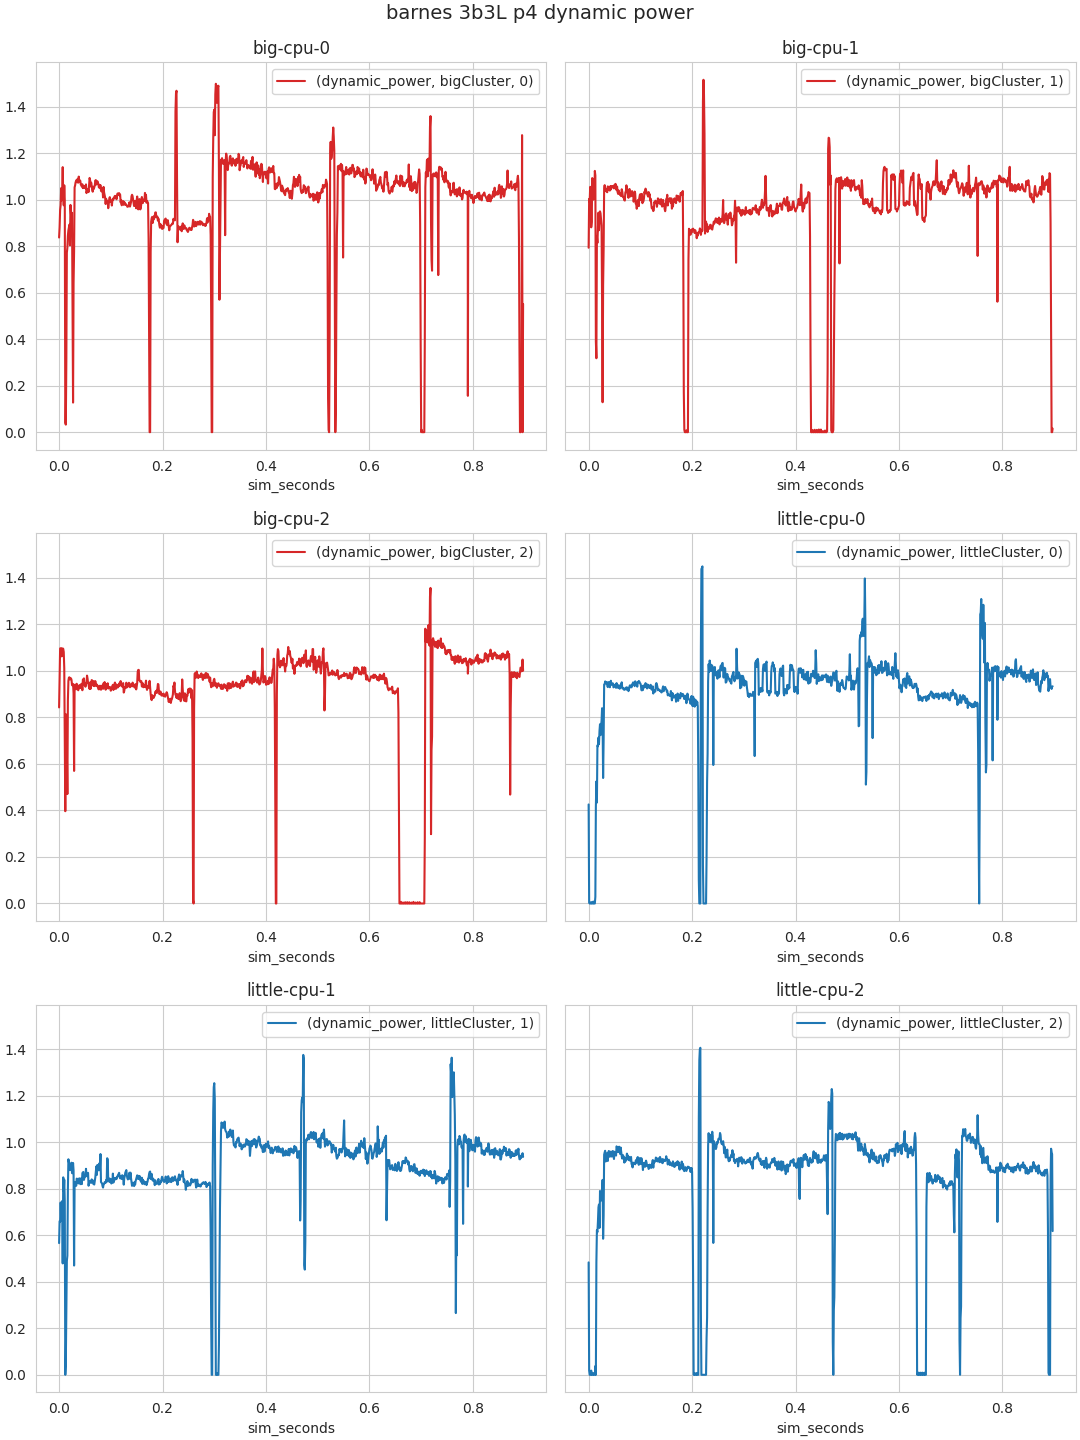
\includegraphics[width=0.8\textwidth]{roi-plots/barnes/3b3L/p4-success-dyn-pow.png}
    \caption{Dynamic power for 4-threaded \texttt{barnes} on 3 big and 3 LITTLE 
             cores (completed)}
\end{figure}

\begin{figure}[H]
    \centering
    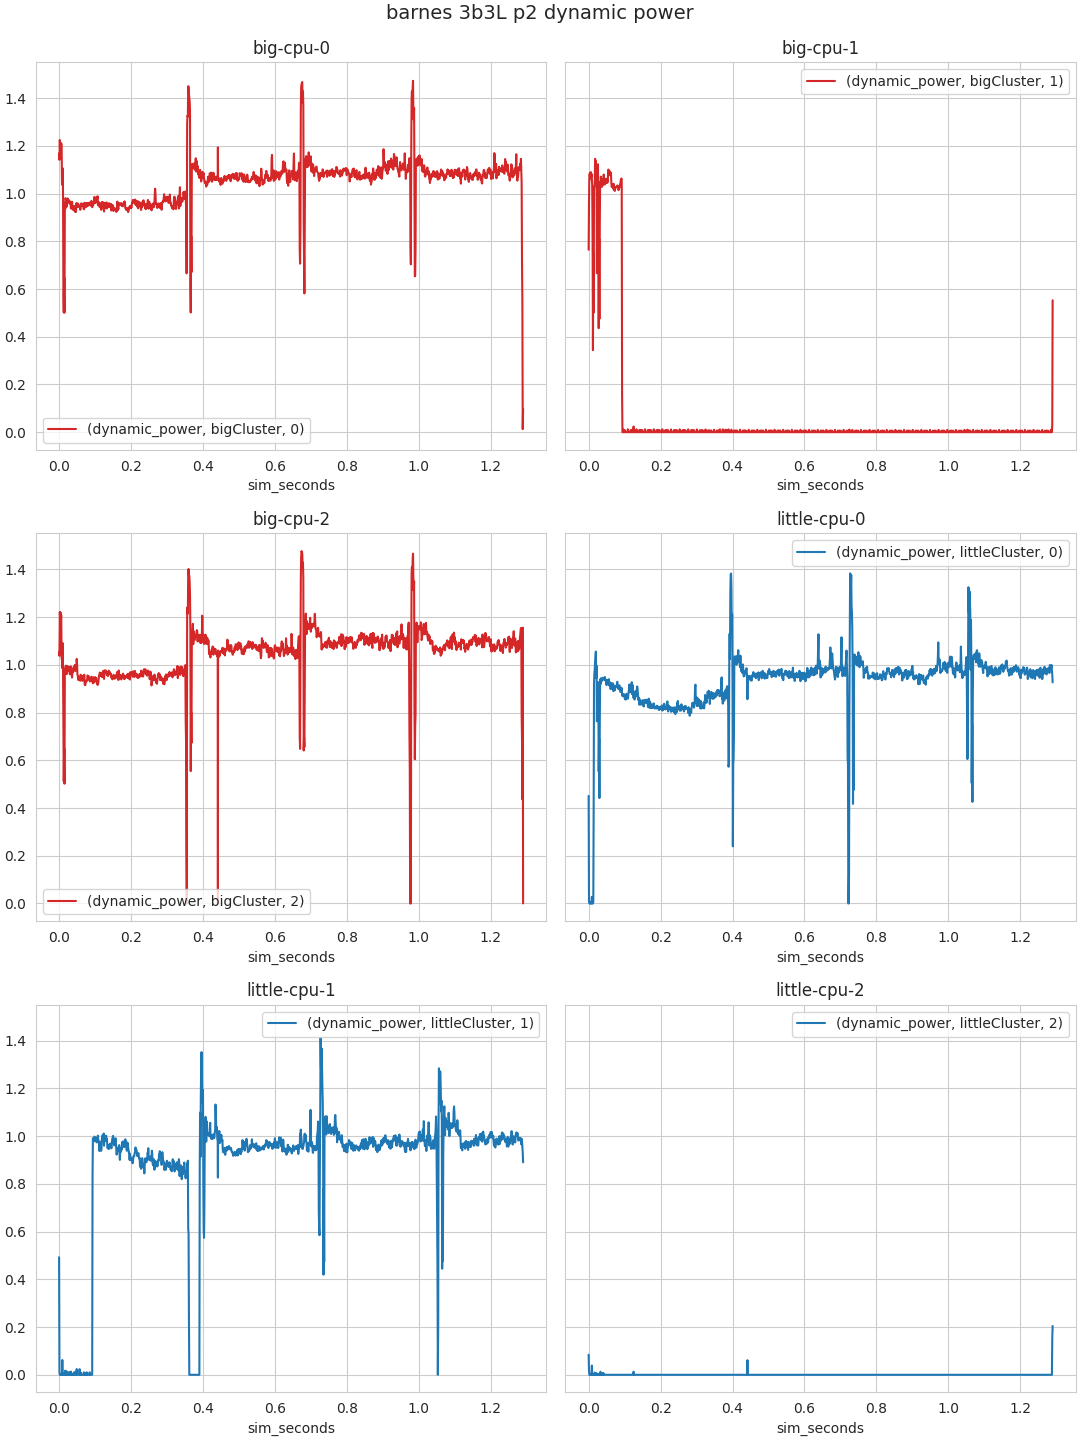
\includegraphics[width=0.8\textwidth]{roi-plots/barnes/3b3L/p2-fail-dyn-pow.png}
    \caption{Dynamic power for 2-threaded \texttt{barnes} on 3 big and 3 LITTLE 
             cores (crashed)}
\end{figure}

\begin{figure}[H]
    \centering
    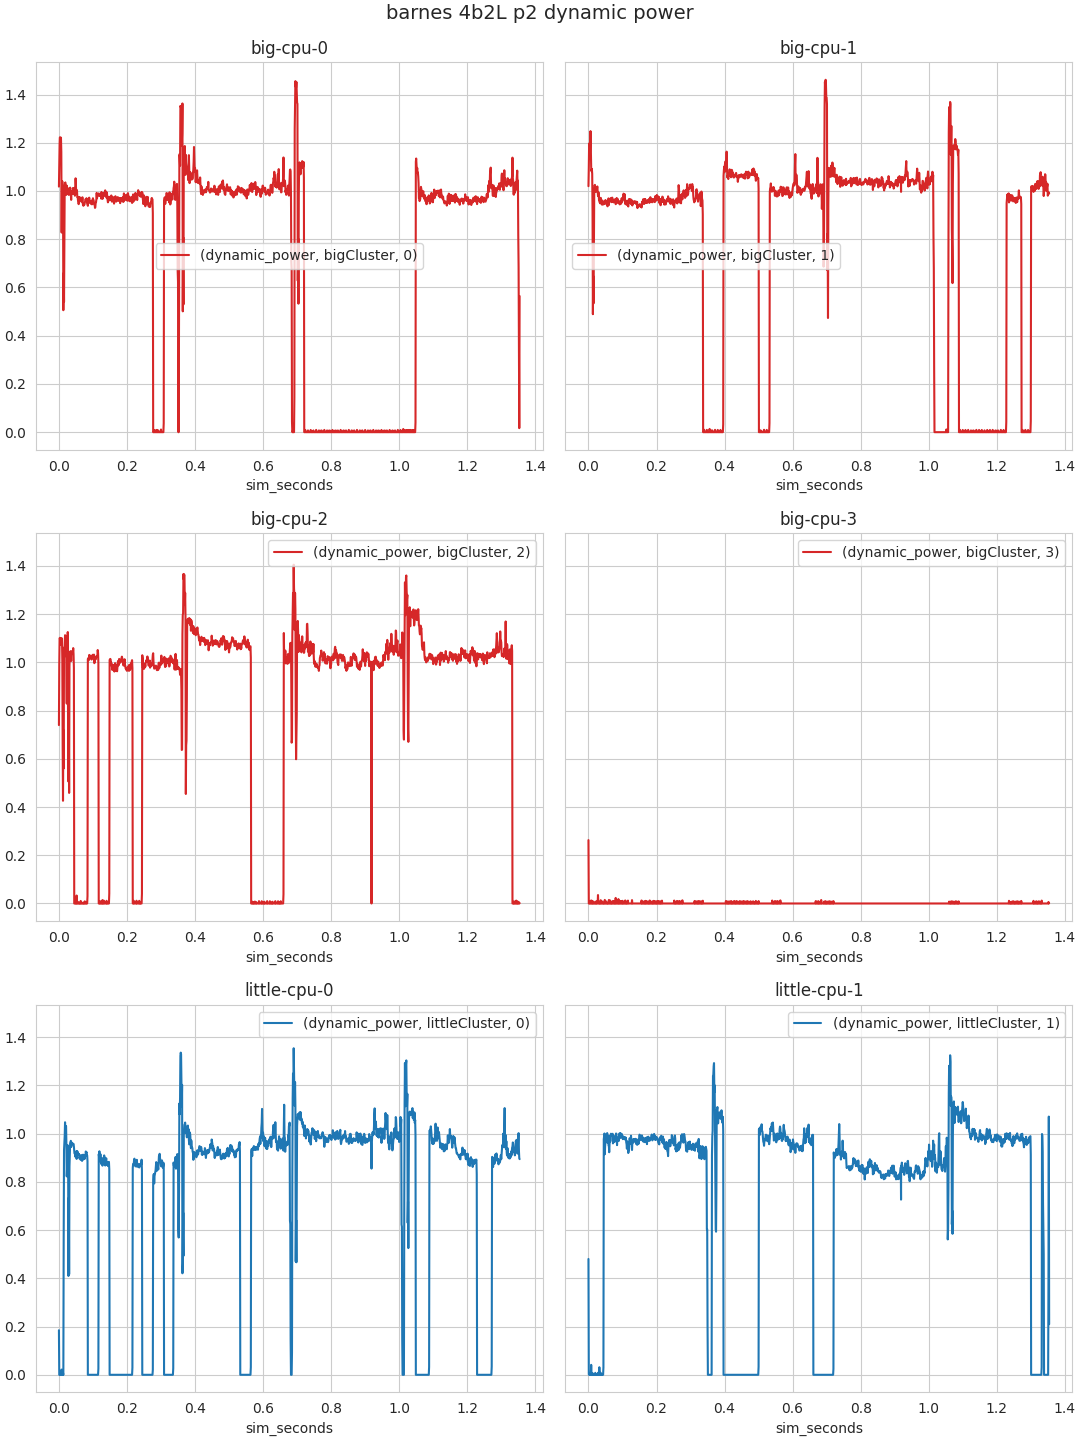
\includegraphics[width=0.8\textwidth]{roi-plots/barnes/4b2L/p2-success-dyn-pow.png}
    \caption{Dynamic power for 2-threaded \texttt{barnes} on 4 big 2 LITTLE
             cores (completed)}
\end{figure}

\begin{figure}[H]
    \centering
    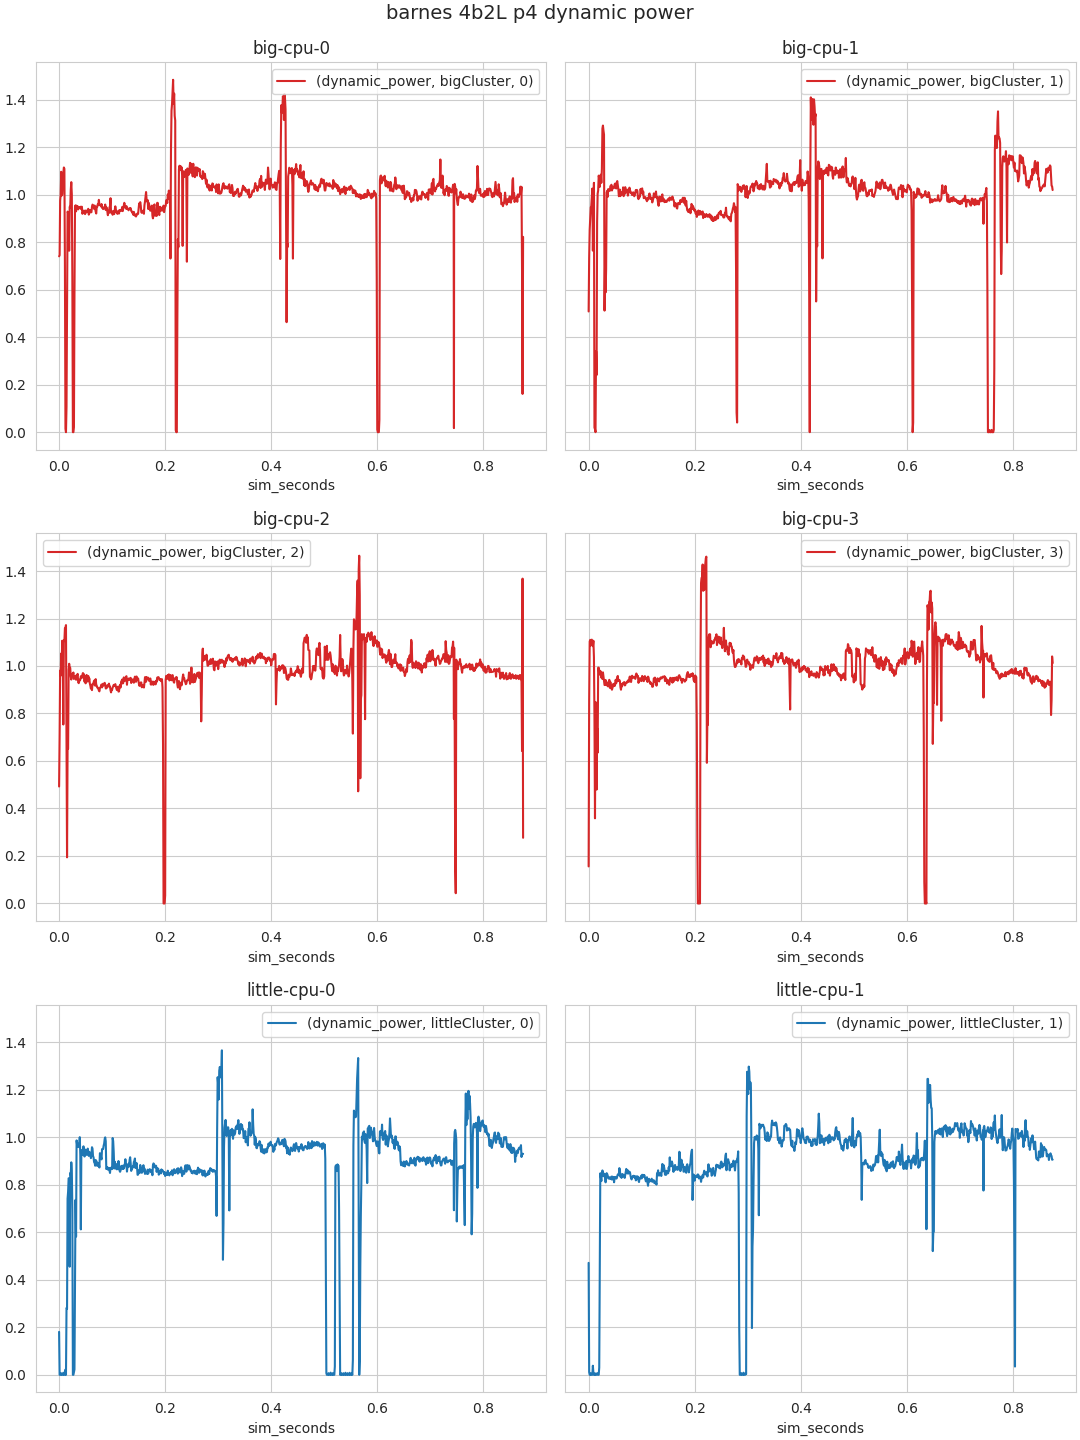
\includegraphics[width=0.8\textwidth]{roi-plots/barnes/4b2L/p4-fail-dyn-pow.png}
    \caption{Dynamic power for 4-threaded \texttt{barnes} on 4 big 2 LITTLE
             cores (crashed)}
\end{figure}


\section{The ocean-contiguous\_partitions benchmark}
\begin{figure}[H]
    \centering
    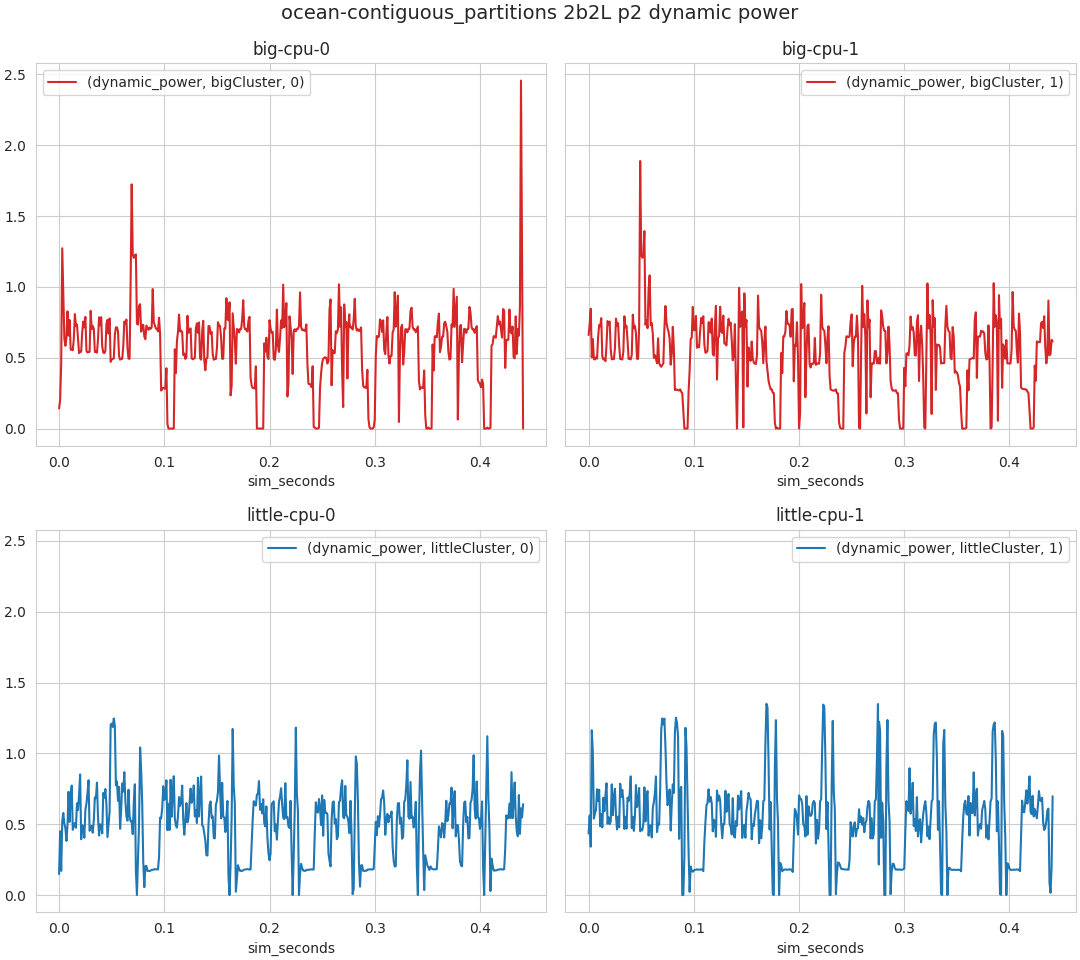
\includegraphics[height=0.6\textheight]{roi-plots/ocean-contiguous/2b2L/p2-success-dyn-pow.png}
    \caption{Dynamic power for 2-threaded \texttt{ocean-contiguous\_partitions}
             on 2 big 2 LITTLE cores (completed)}
\end{figure}

\begin{figure}[H]
    \centering
    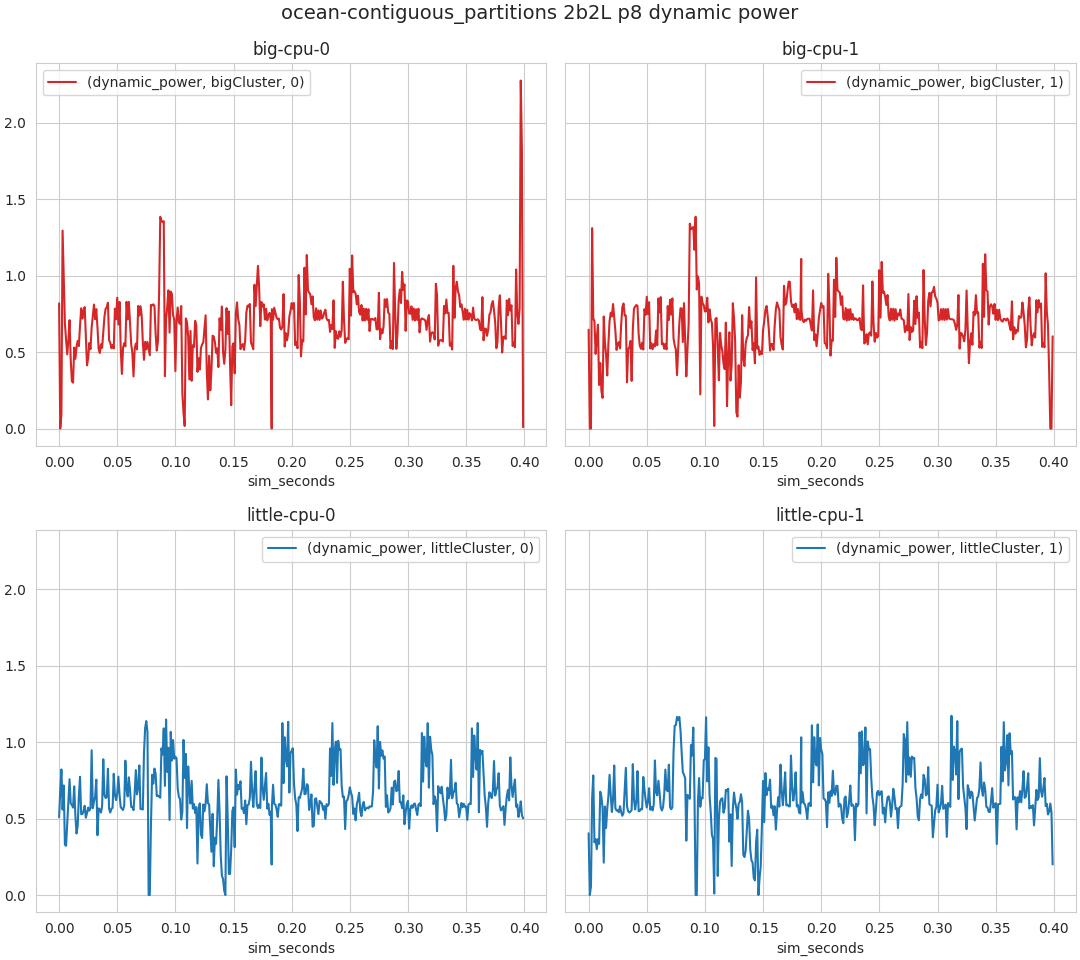
\includegraphics[height=0.6\textheight]{roi-plots/ocean-contiguous/2b2L/p8-fail-dyn-pow.png}
    \caption{Dynamic power for 8-threaded \texttt{ocean-contiguous\_partitions}
             on 2 big 2 LITTLE cores (crashed)}
\end{figure}

\begin{figure}[H]
    \centering
    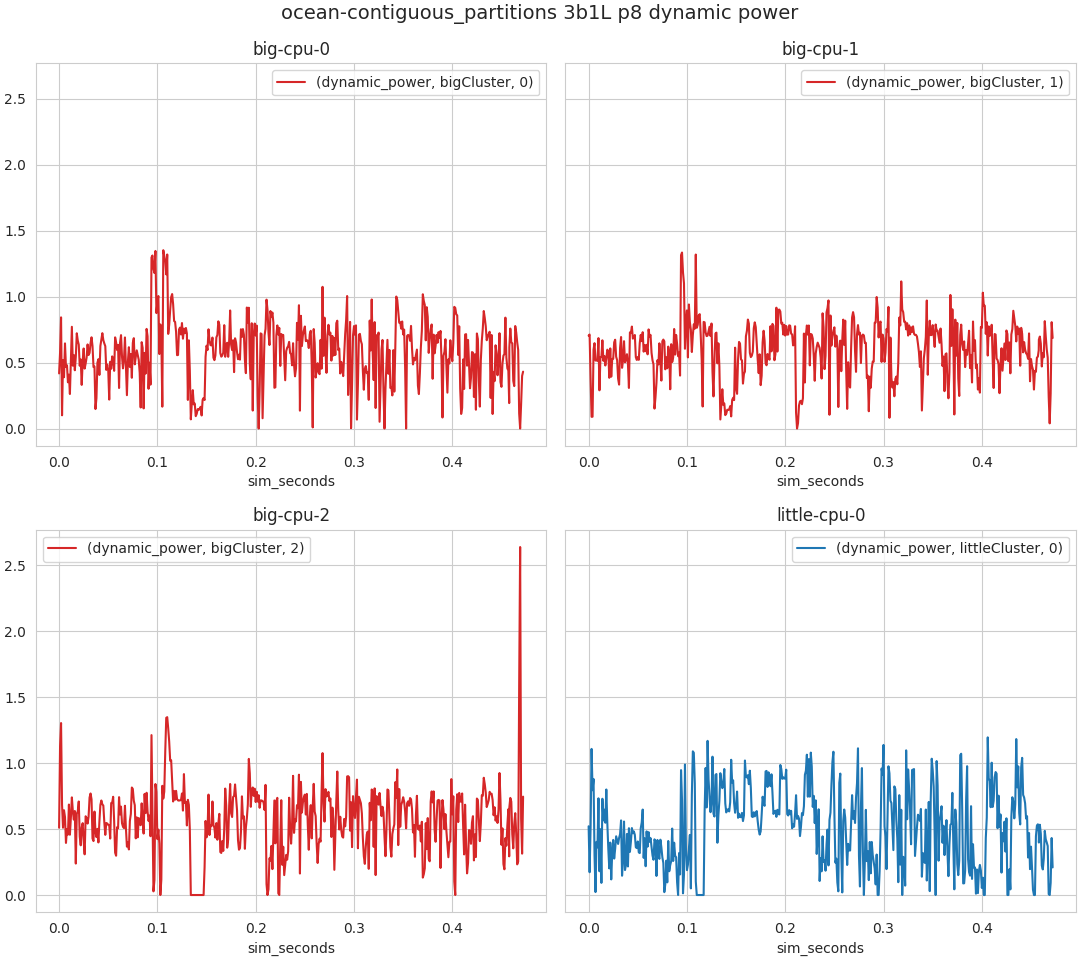
\includegraphics[height=0.6\textheight]{roi-plots/ocean-contiguous/3b1L/p8-success-dyn-pow.png}
    \caption{Dynamic power for 8-threaded \texttt{ocean-contiguous\_partitions}
             on 3 big 1 LITTLE cores (completed)}
\end{figure}

\begin{figure}[H]
    \centering
    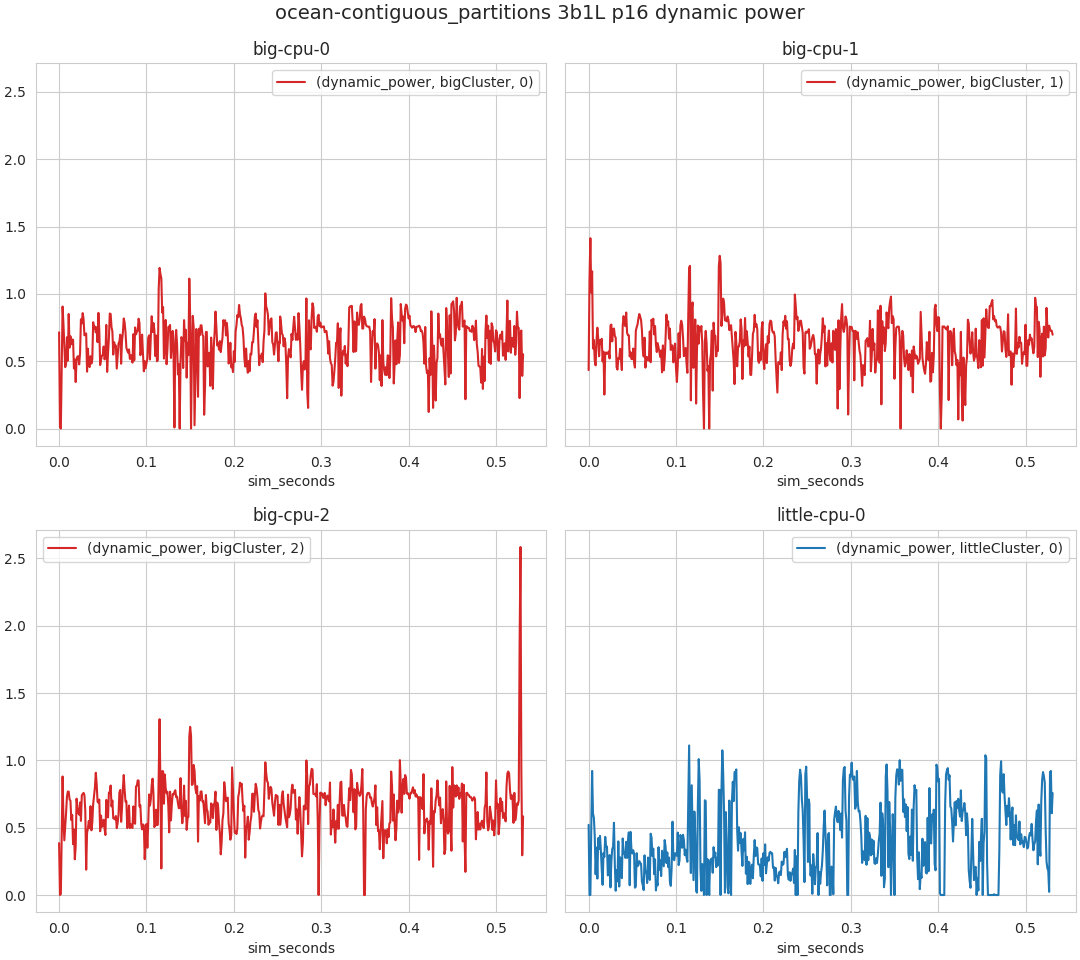
\includegraphics[height=0.6\textheight]{roi-plots/ocean-contiguous/3b1L/p16-fail-dyn-pow.png}
    \caption{Dynamic power for 16-threaded \texttt{ocean-contiguous\_partitions}
             on 3 big 1 LITTLE cores (crashed)}
\end{figure}


\section{The water-spatial benchmark}
\begin{figure}[H]
    \centering
    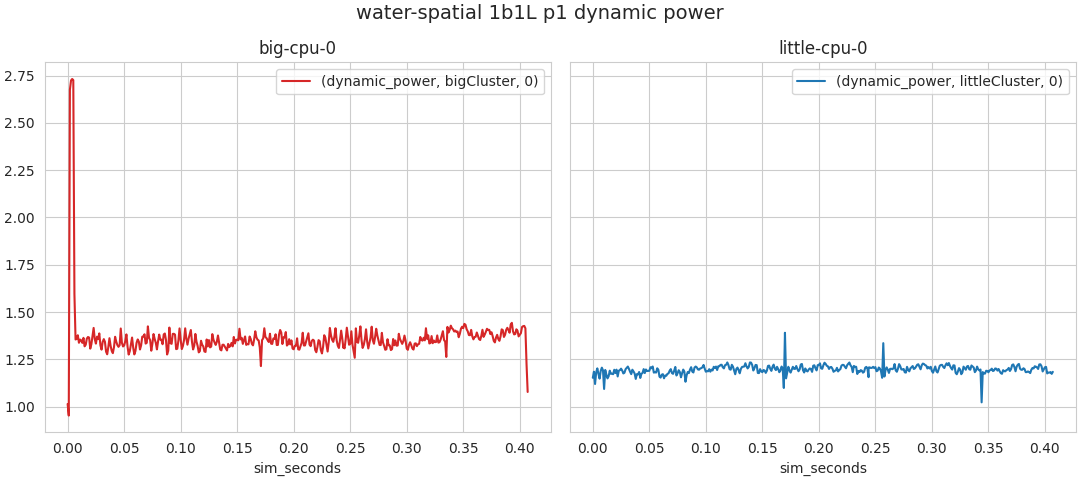
\includegraphics[width=0.9\textwidth]{roi-plots/water-spatial/1b1L/p1-success-dyn-pow.png}
    \caption{Dynamic power for single-threaded \texttt{water-spatial} on 1 big
             1 LITTLE core (completed)}
\end{figure}

\begin{figure}[H]
    \centering
    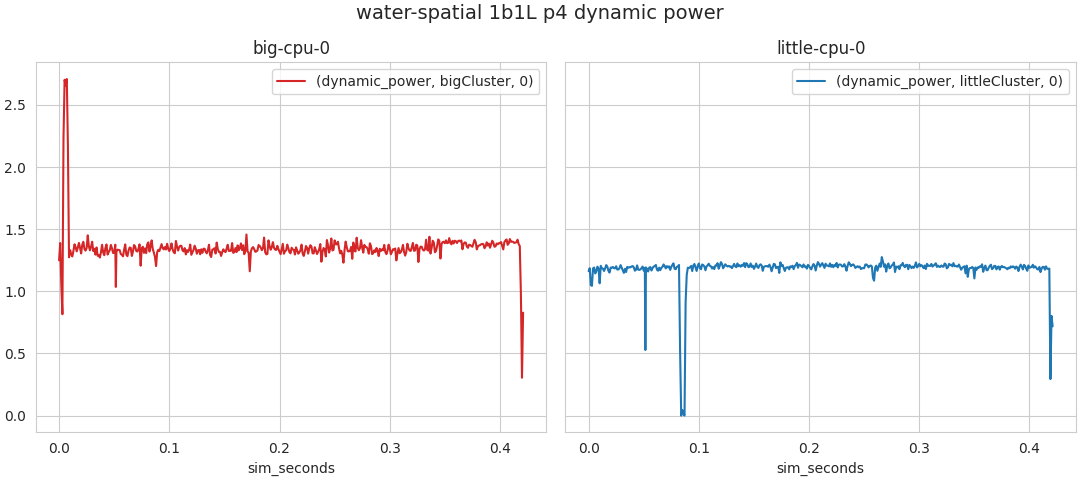
\includegraphics[width=0.9\textwidth]{roi-plots/water-spatial/1b1L/p4-fail-dyn-pow.png}
    \caption{Dynamic power for 4-threaded \texttt{water-spatial} on 1 big 1
             1 LITTLE core (crashed)}
\end{figure}

\begin{figure}[H]
    \centering
    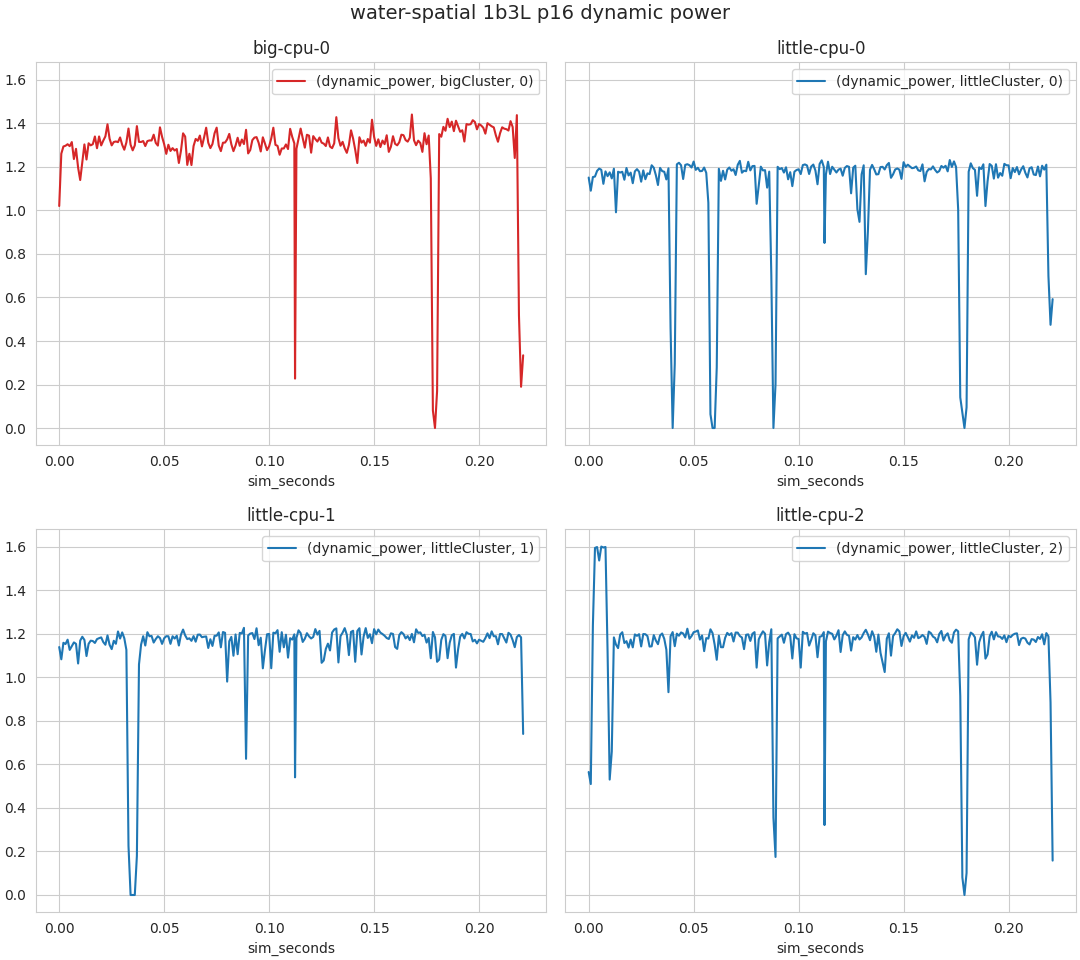
\includegraphics[height=0.6\textheight]{roi-plots/water-spatial/1b3L/p16-success-dyn-pow.png}
    \caption{Dynamic power for 16-threaded \texttt{water-spatial} on 1 big 3
             LITTLE cores (completed)}
\end{figure}

\begin{figure}[H]
    \centering
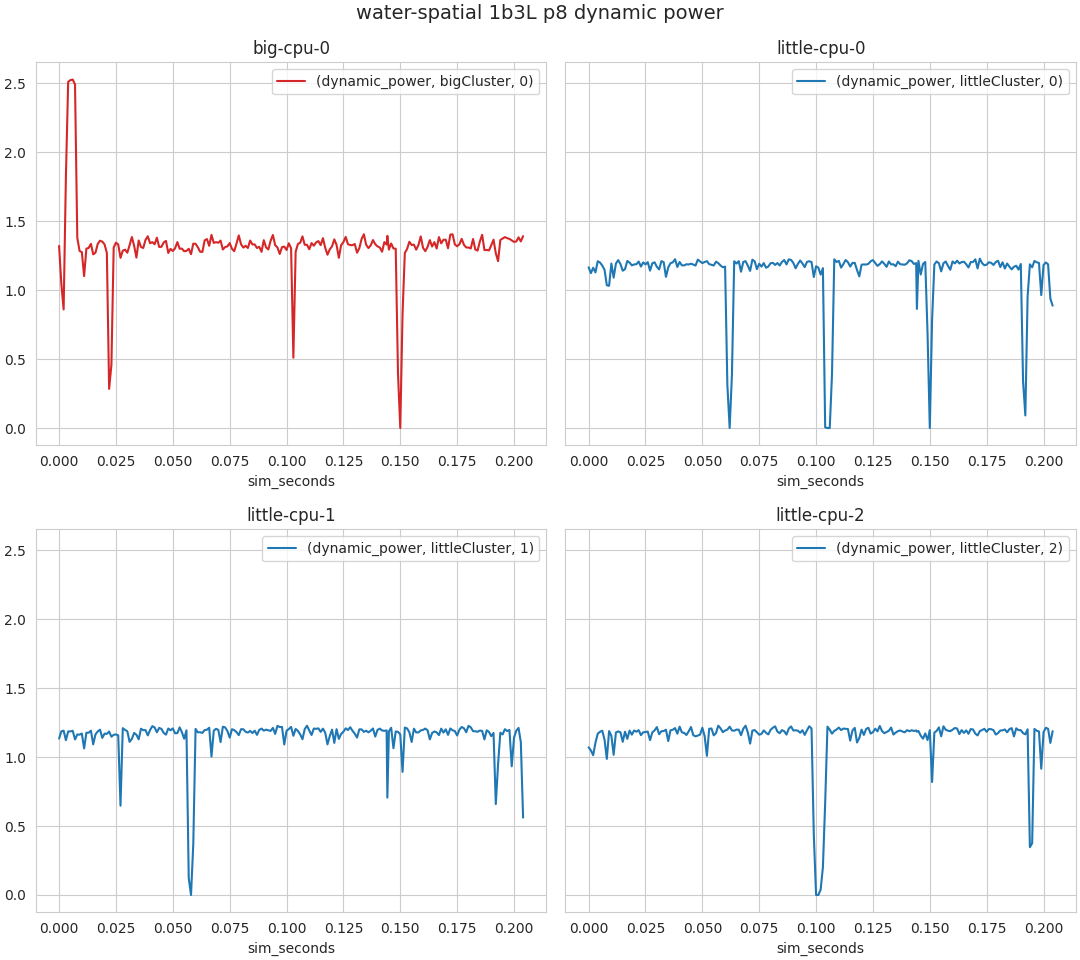
\includegraphics[height=0.6\textheight]{roi-plots/water-spatial/1b3L/p8-fail-dyn-pow.png}
\caption{Dynamic power for 8-threaded \texttt{water-spatial} on 1 big 3
         LITTLE cores (crashed)}
\end{figure}
